\documentclass[UTF8,zihao=-4]{ctexbeamer}
\usepackage{multimedia}
\usepackage{hyperref}

\usepackage{listings}

%% 所要粘贴代码的编程语言
%\lstloadlanguages{}

%% 设置listings宏包的一些全局样式
%% 参考http://hi.baidu.com/shawpinlee/blog/item/9ec431cbae28e41cbe09e6e4.html
\lstset{
	showstringspaces=false,              %% 设定是否显示代码之间的空格符号
	numbers=left,                        %% 在左边显示行号
	numberstyle=\tiny,                   %% 设定行号字体的大小
	basicstyle=\footnotesize,                    %% 设定字体大小\tiny, \small, \Large等等
	keywordstyle=\color{blue!70}, commentstyle=\color{red!50!green!50!blue!50},
	%% 关键字高亮
	frame=shadowbox,                     %% 给代码加框
	rulesepcolor=\color{red!20!green!20!blue!20},
	escapechar=`,                        %% 中文逃逸字符,用于中英混排
	xleftmargin=2em,xrightmargin=2em, aboveskip=1em,
	breaklines,                          %% 这条命令可以让LaTeX自动将长的代码行换行排版
	extendedchars=false                  %% 这一条命令可以解决代码跨页时,章节标题,页眉等汉字不显示的问题
}

\usetheme{Madrid}
%\useoutertheme{miniframes}

\usecolortheme{orchid}
\title{基本指令(二)}
\author{高星}
\institute{湖南潇湘技师学院~湖南九嶷职院}
\date{2017.09.21}
\begin{document}
    
\begin{frame}[plain]
		\maketitle
\end{frame}

\begin{frame}
\begin{columns}
\column[t]{0.3\textwidth}
\column[t]{0.7\textwidth}
\tableofcontents[hideallsubsections]
\end{columns}
\end{frame}

\section*{教学目标}

\begin{frame}{教学目标}
    \begin{columns}
        \column{.2\textwidth}
        \column{.8\textwidth}
        \begin{enumerate}
	\item 掌握G2/G3半径-R的使用;
\item 掌握G2/G3圆心编程的使用;
\item 能用G2/G3进行程序的编写;
\item 掌握编写数控程序的基本思路。
        \end{enumerate}
    \end{columns}
\end{frame}

\section{案例分析-复习}
\begin{frame}{复习案例}
     \begin{columns}
        \column{.4\textwidth}
        在数控铣床或加工中心上加工如图所示的零件,试完成程序的编写,已知毛坯为 $\Phi$ 110*30。
        \column{.6\textwidth}

\begin{figure}
    \centering
    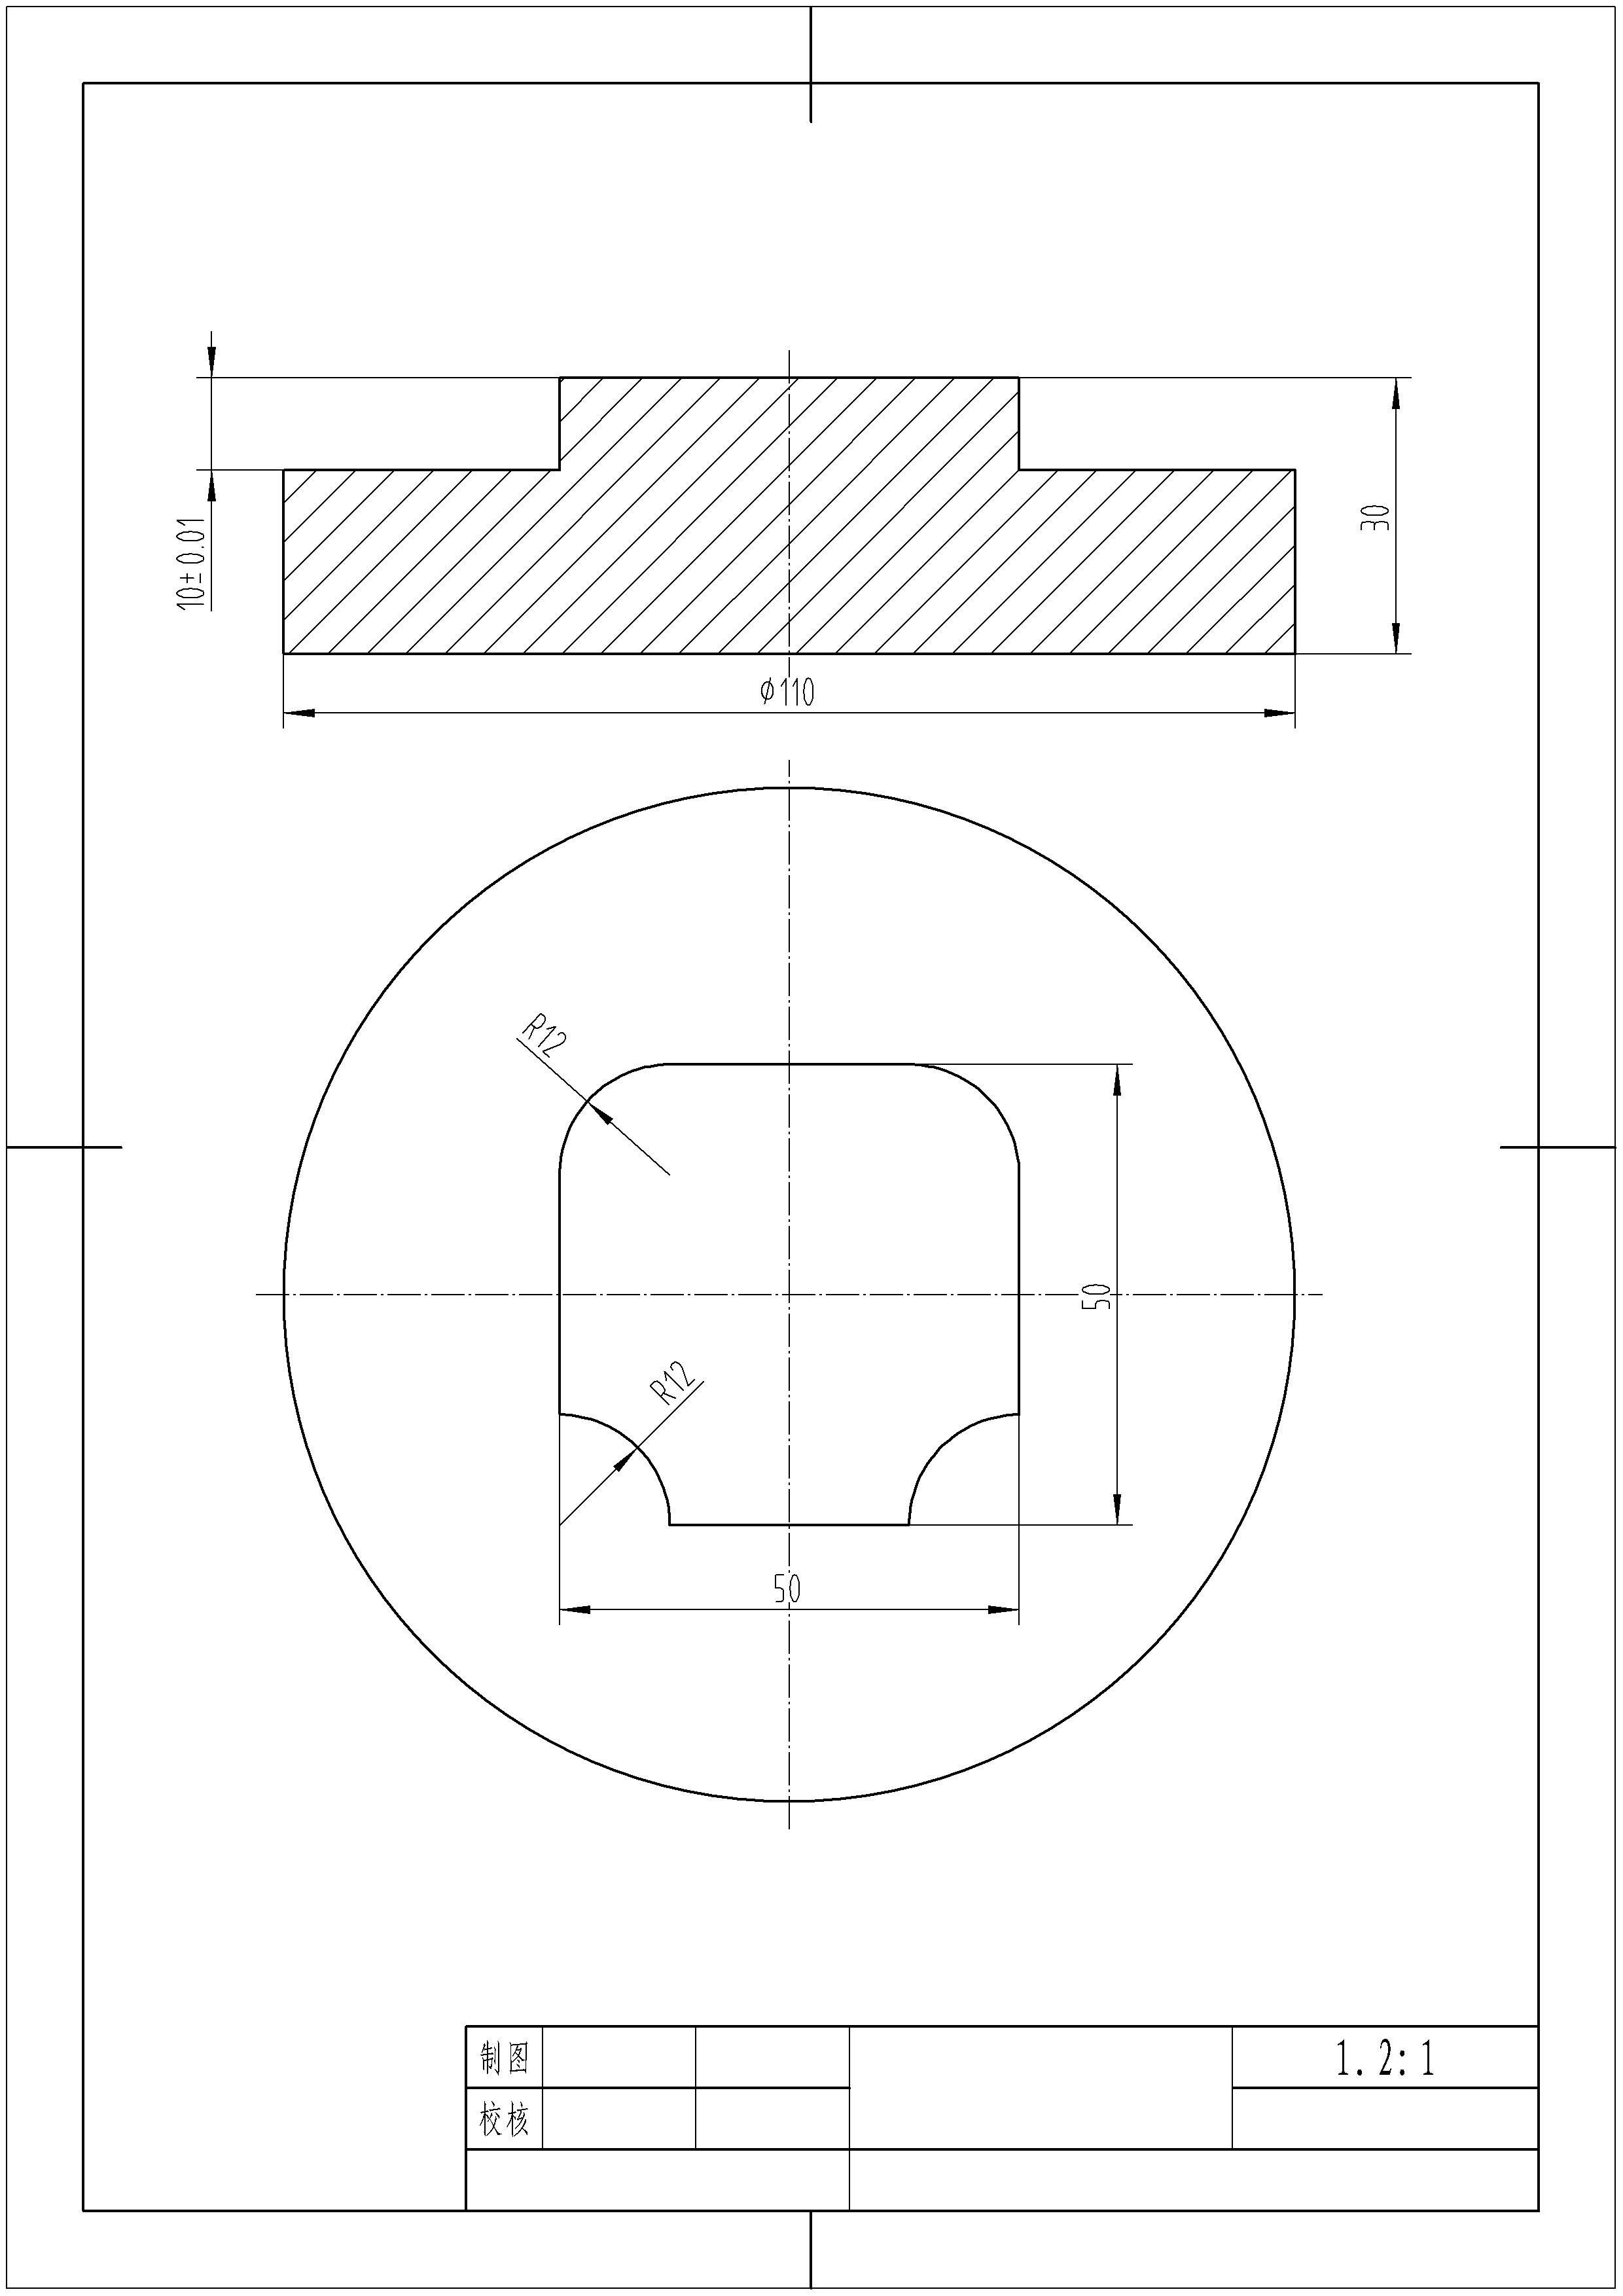
\includegraphics[width=0.8\linewidth,trim=50 150 50 100,clip]{image/5-1.jpg}
%    \caption{}
    \label{fig:5-1}
\end{figure}
    \end{columns}
\end{frame}

\begin{frame}{手工编程流程}
    \begin{columns}
        \column{.2\textwidth}
        \column{.8\textwidth}
\begin{enumerate}
    \item 图样分析;
    \item 确定加工内容;
    \item 确定装夹及工件坐标系;
    \item 确定刀具及切削用量;
    \item 确定工序及走刀路线;
    \item 计算点坐标;
    \item 编写程序单。
\end{enumerate}
    \end{columns}
\end{frame}

\section{-R案例}
\begin{frame}{-R案例}
    \begin{columns}
        \column{.4\textwidth}
        在数控铣床或加工中心上加工如图所示的零件,试完成程序的编写,已知毛坯为 $\Phi$ 110*30。
        \column{.6\textwidth}
        
        \begin{figure}
            \centering
            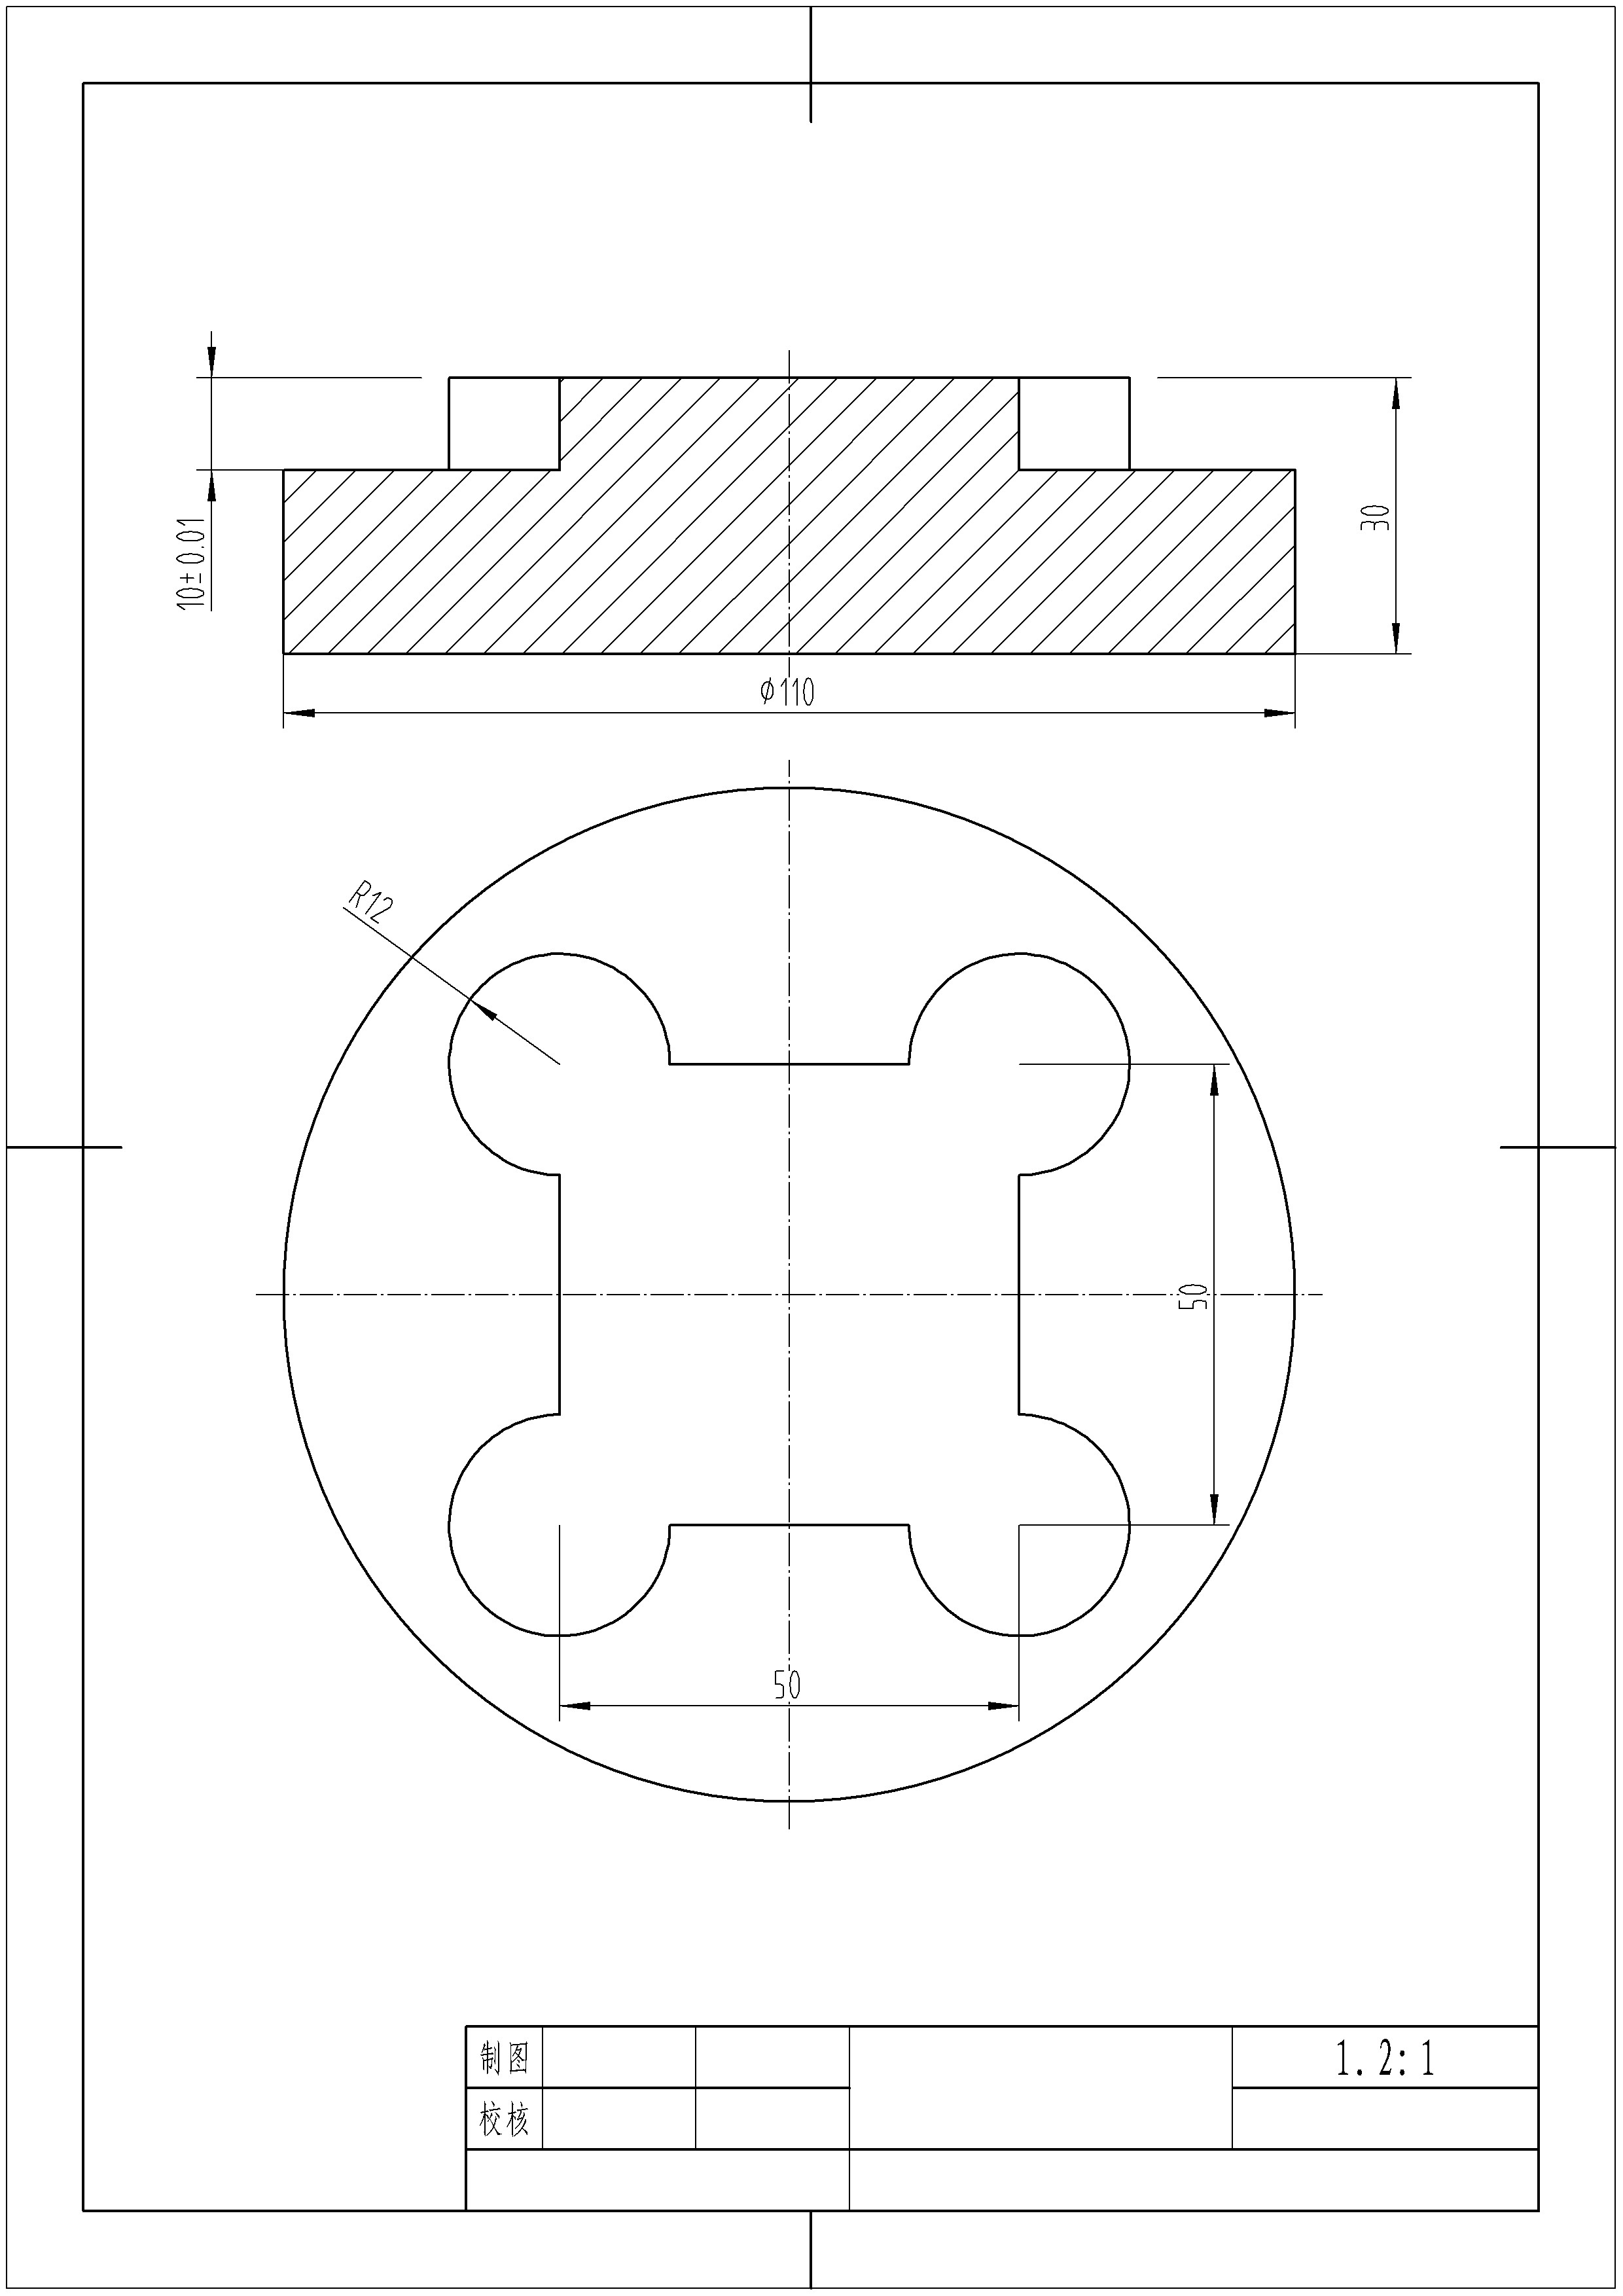
\includegraphics[width=0.8\linewidth,trim=50 150 50 100,clip]{image/5-2.jpg}
            %    \caption{}
            \label{fig:5-2}
        \end{figure}
    \end{columns}
\end{frame}

\begin{frame}{手工编程流程}
    \begin{columns}
        \column{.0\textwidth}
        \column{\textwidth}
        
        路径特点:
        
        圆弧的圆心角大于180度,显然不能直接用前面的程序。
        
        解决方法:
        
        
        1、把圆弧分成多个圆心角小于180度的圆弧。
        
        2、使用圆心角大于180度圆弧指令的使用。
        
              
        当圆心角大于180度时,用负的半径值来表示。
        
        当圆心角小于180度时,用正的半径值来表示。
        
        Siemens上用CR= 正负规则一样。
        
    \end{columns}
\end{frame}

\section{整圆案例}
\begin{frame}{整圆案例}
    \begin{columns}
        \column{.4\textwidth}
        在数控铣床或加工中心上用整圆的路径进行面铣,面铣深度为1mm,试完成加工成型的编写,已知毛坯为 $\Phi$ 110*30。
        \column{.6\textwidth}
        
        \begin{figure}
            \centering
            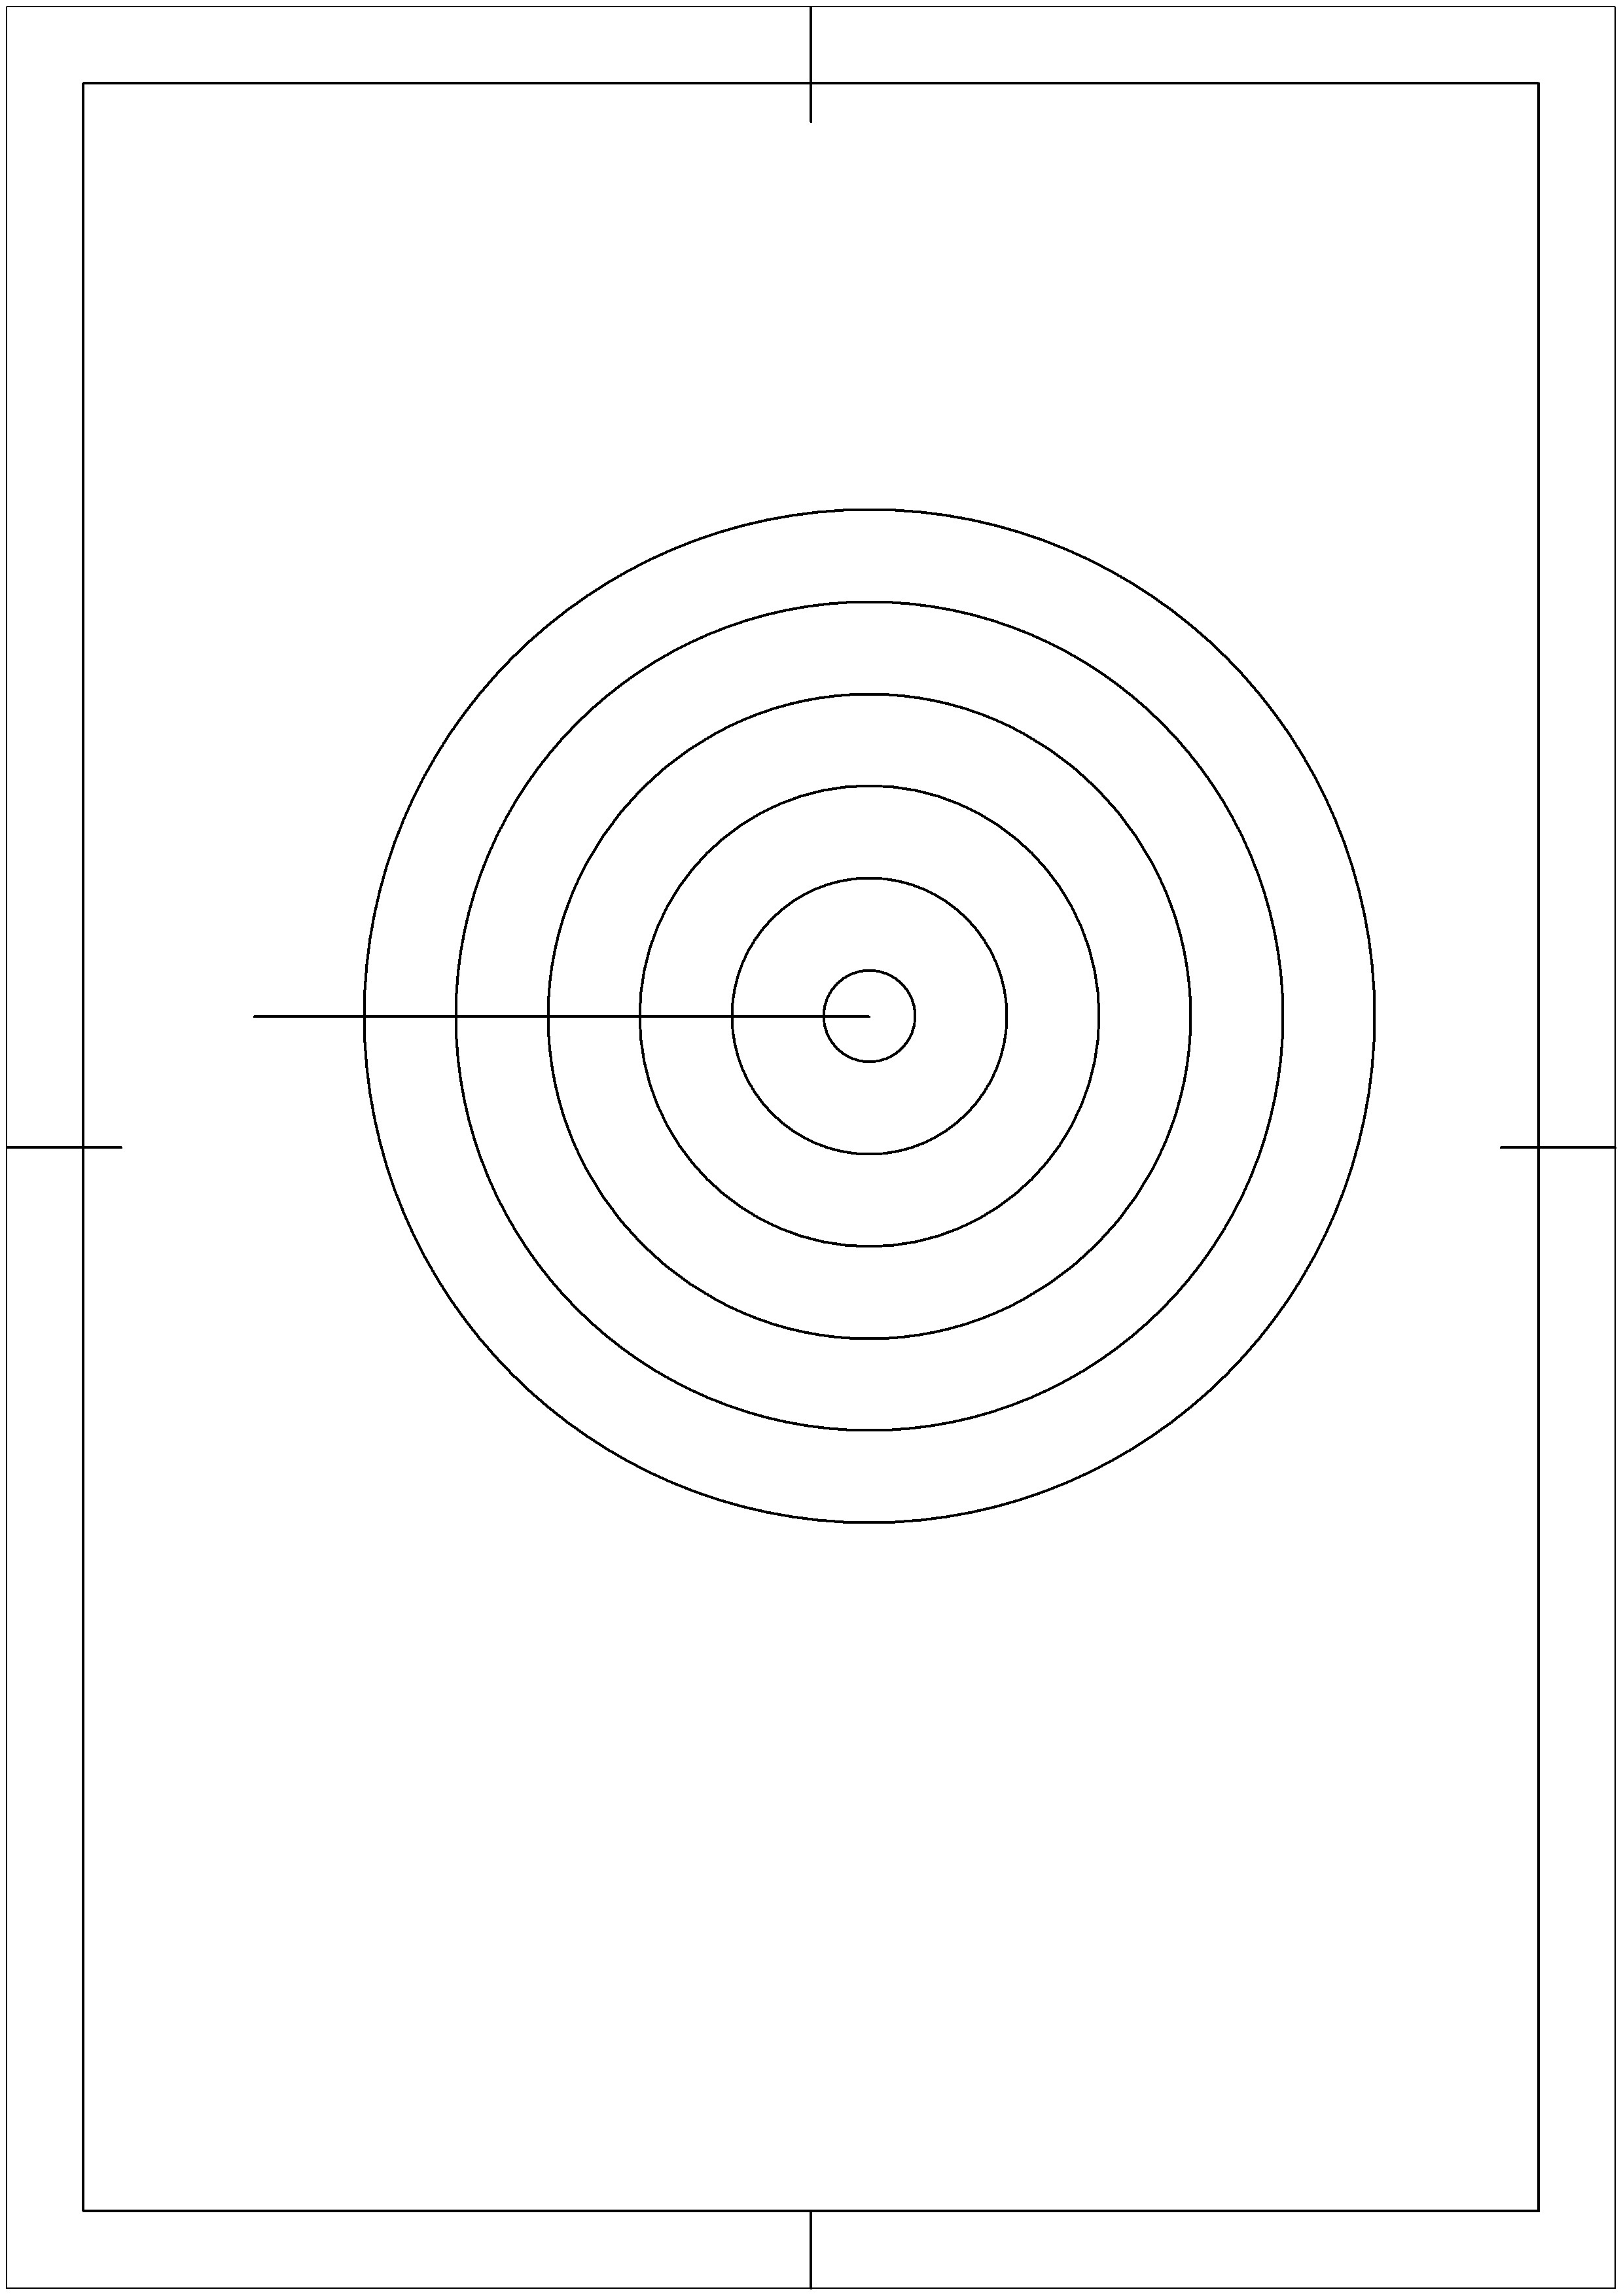
\includegraphics[width=0.8\linewidth,trim=50 150 50 100,clip]{image/5-3.jpg}
            %    \caption{}
            \label{fig:5-3}
        \end{figure}
    \end{columns}
\end{frame}





\section{I、J、K的应用}
\begin{frame}{整圆案例}
    \begin{columns}
        \column{.4\textwidth}
        在数控铣床或加工中心上加工如图所示的零件,试用I、J、K完成程序的编写,已知毛坯为 $\Phi$ 110*30。
        \column{.6\textwidth}
        
        \begin{figure}
            \centering
            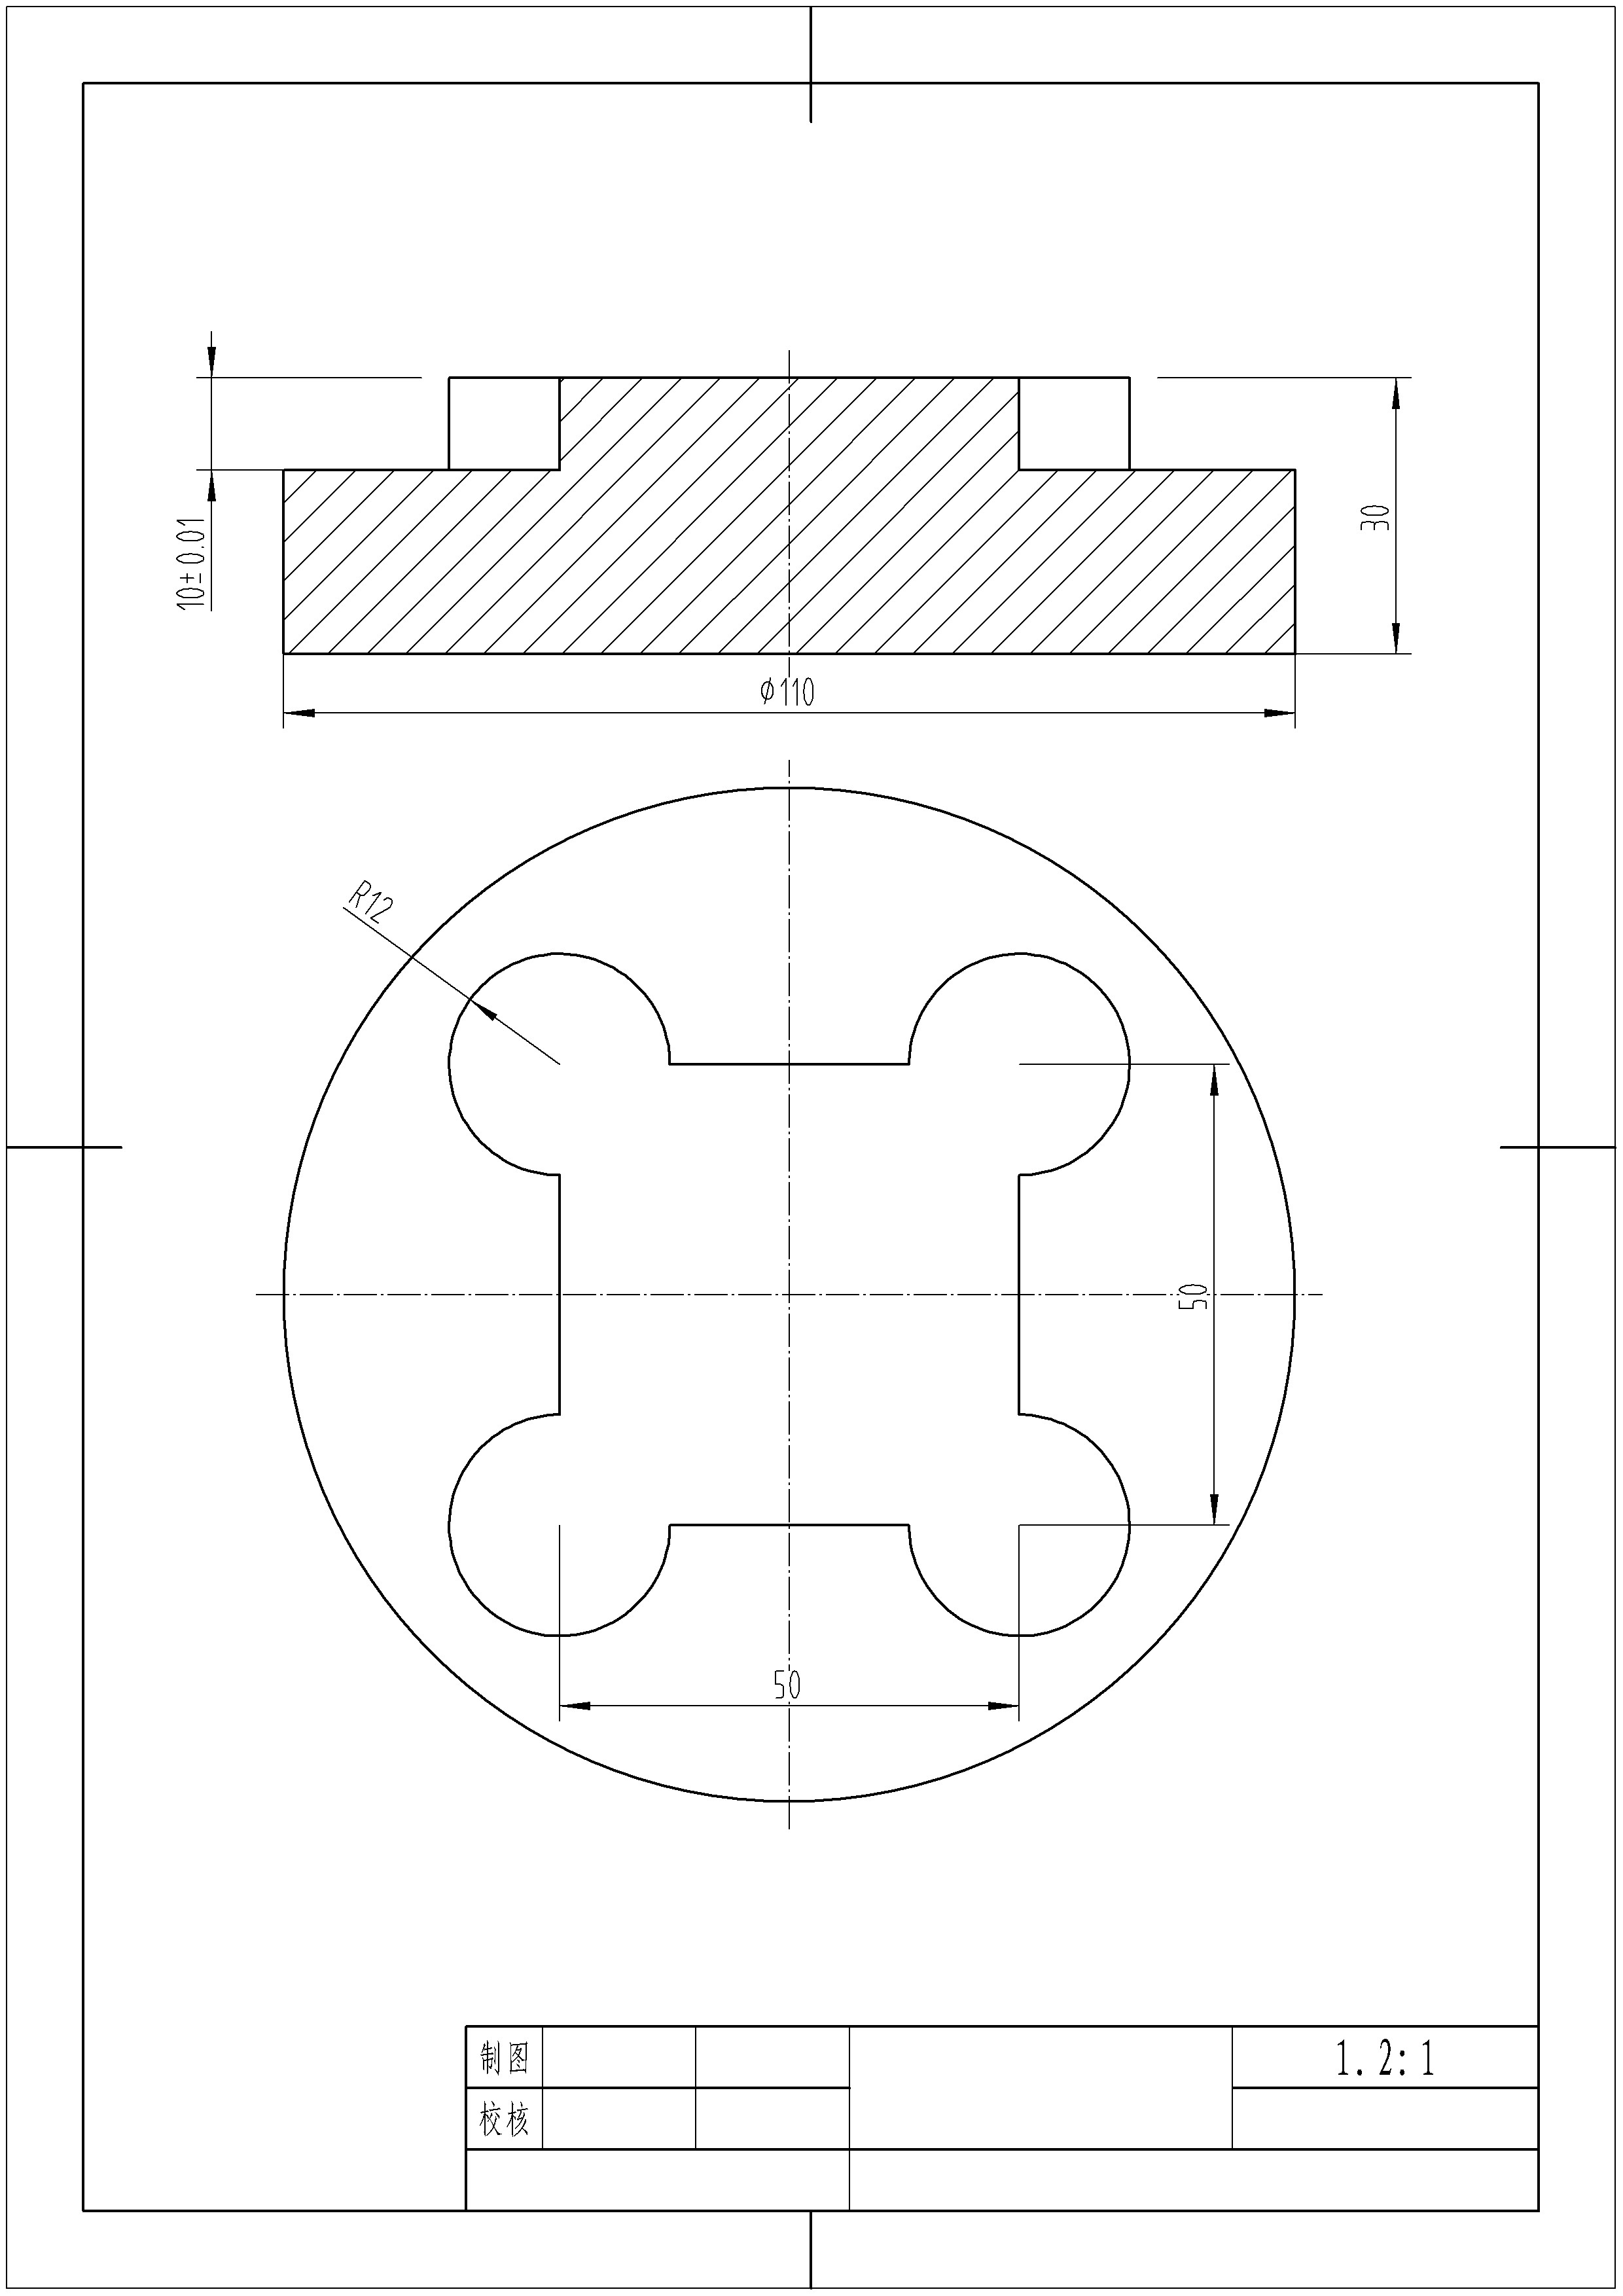
\includegraphics[width=0.8\linewidth,trim=50 150 50 100,clip]{image/5-4.jpg}
            %    \caption{}
            \label{fig:5-4}
        \end{figure}
    \end{columns}
\end{frame}


\section{编写程序的基本思路}
\begin{frame}{零件编程}
    \begin{columns}
        \column{.0\textwidth}
        \column{\textwidth}
 程序初始化(安全保护)--------辅助准备(换刀,主轴启动,切削液开)--------定位到起刀点--------快速下刀--------工进下刀--------走加工轮廓--------提刀---------快速提刀到安全平面-------程序结束(换刀,主轴停止,切削液关,程序返回等)       
        
    \end{columns}
\end{frame}



\section*{课堂小结}
\begin{frame}{课堂小结}
    \begin{columns}
        \column{.2\textwidth}
        \column{.8\textwidth}
\begin{enumerate}
\item 圆心角大于180度的圆弧指令。
\item 圆弧的圆心编程。
\item 编程实例。
\item 编写程序的基本思路
\end{enumerate}
    \end{columns}
\end{frame}

\begin{frame}{作业}
\begin{enumerate}
    \item 自定尺寸,编写加工一个圆弧凸台的数控程序。
\end{enumerate}
\end{frame}

\begin{frame}[plain]
\vfill

\centering \huge 谢谢大家!

\vfill

\flushleft \footnotesize   
~~~QQ:32731964\\
~~~TEL:18974681118\\
%~~~课件下载:\\
%~~~https://github.com/gnixoag/myworks2017/tree/master/jiaoshichengzhang

\end{frame}

\end{document} 
